\documentclass{beamer}

%Russian-specific packages
%--------------------------------------
\usepackage[T2A]{fontenc}
\usepackage[utf8]{inputenc}
\usepackage[russian]{babel}
%--------------------------------------

\usepackage{booktabs}
\usepackage{graphicx}

\title{Оптимизация функции, задаваемой регрессионным лесом}
\author{Влад Ягламунов}
\date{}

\begin{document}

\maketitle

\begin{frame}
\frametitle{Алгоритм}
\begin{columns}
    \column{.5\textwidth}
    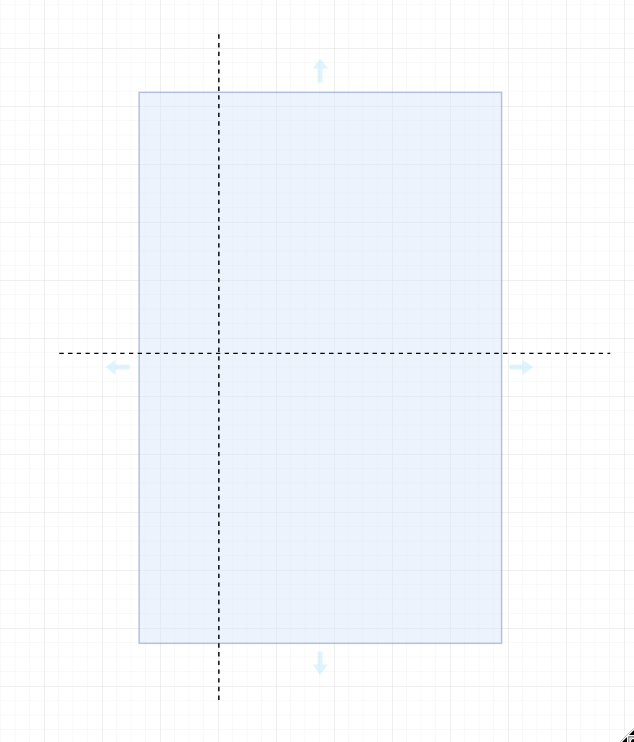
\includegraphics[width=\textwidth]{split.png}
    \column{.5\textwidth}
    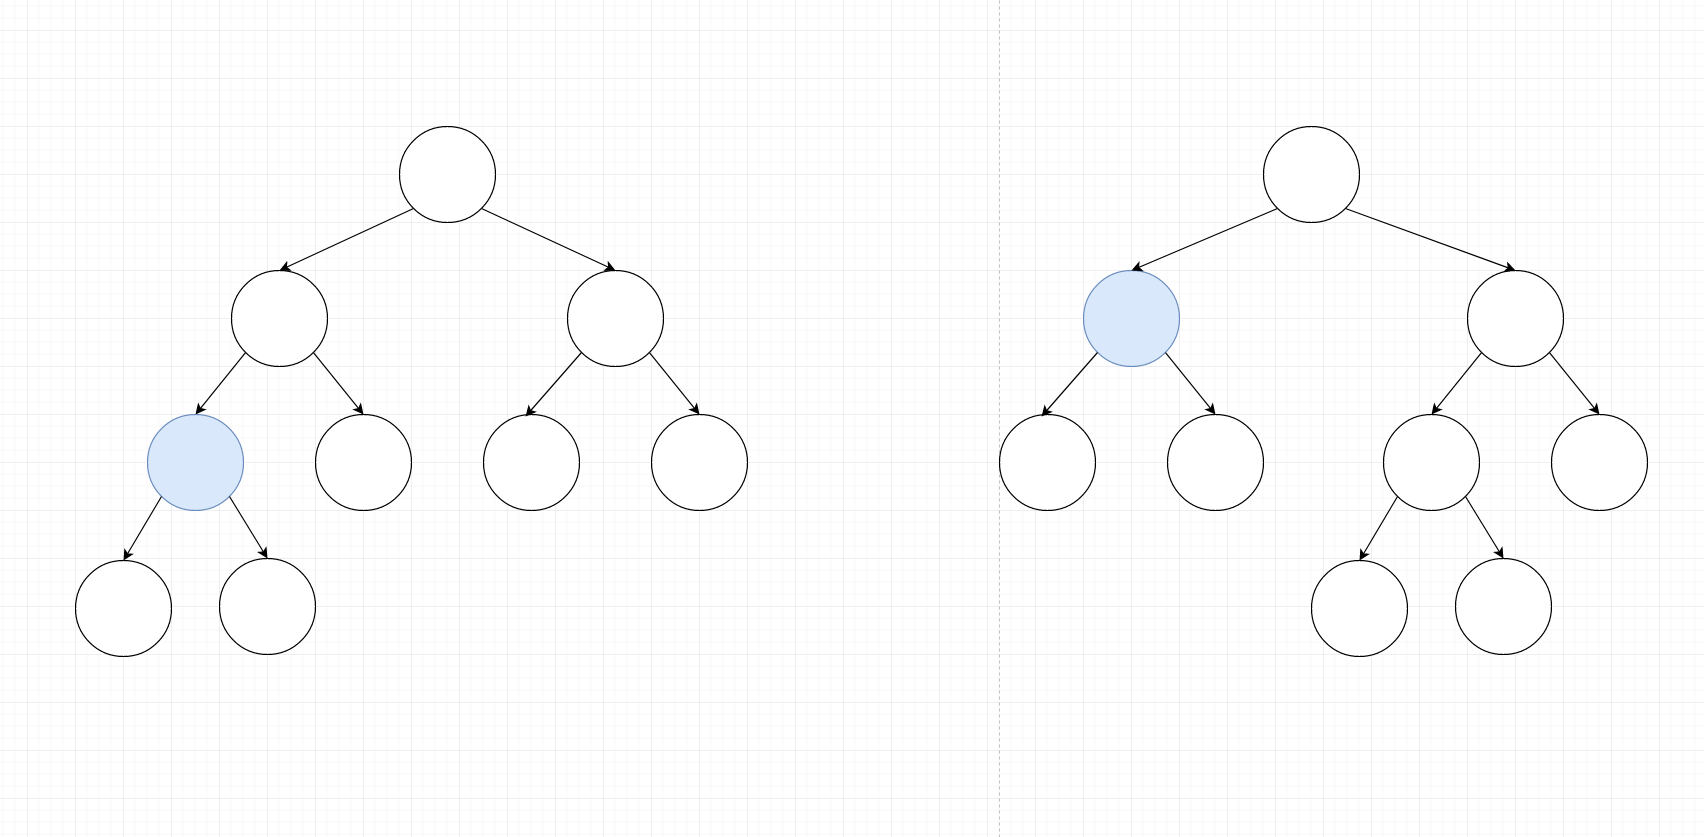
\includegraphics[width=\textwidth]{tree.png}
\end{columns}
\end{frame}

\begin{frame}
\frametitle{Алгоритм}
    \begin{center}
    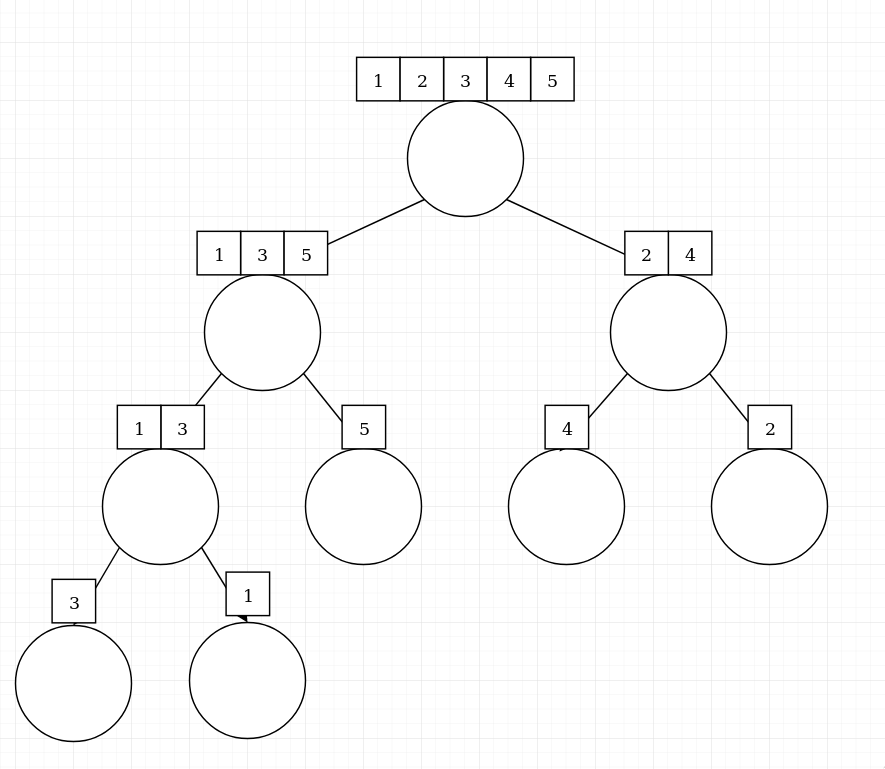
\includegraphics[height=0.8\textheight]{merge.png}
    \end{center}
\end{frame}

\begin{frame}
\frametitle{Тестирование}

\hspace*{-0.8cm}
    \begin{tabular}{l l l l l l l}

        название        & элементы  & признаки & N & время & N & время \\

        \toprule

        diabetes        & 442    & 9     & 30 & 1.07  & 50       & 20\\
                        &        &       & 30+5\% & 0.24  & 50+5\%      & 5\\
        boston          & 506    & 12    & 30 & 0.27  & 100      & 1\\
        autoPrice       & 159    & 16    & 30 & 0.01  & 100      & 6\\
        wisconsin       & 194    & 33    & 30 & 17    & 30+5\%   & 55\\
        strikes         & 625    & 7     & 30 & 0.3   & 100      & 1.5\\
        kin8nm          & 8192   & 9     & 30 & 176   & 30+5\%   & 77\\
        house\_8L       & 22784  & 9     & 30 & 30    & 30+5\%   & 29\\
        house\_16H      & 22784  & 9     & 20 & 112   & 20+5\%   & 55\\
        mtp2            & 274    & 1143  & 30 & 0.30  & 60       & 1.0\\

    \end{tabular}
\hspace*{-0.8cm}


\end{frame}

\begin{frame}
\frametitle{Сравнение}
    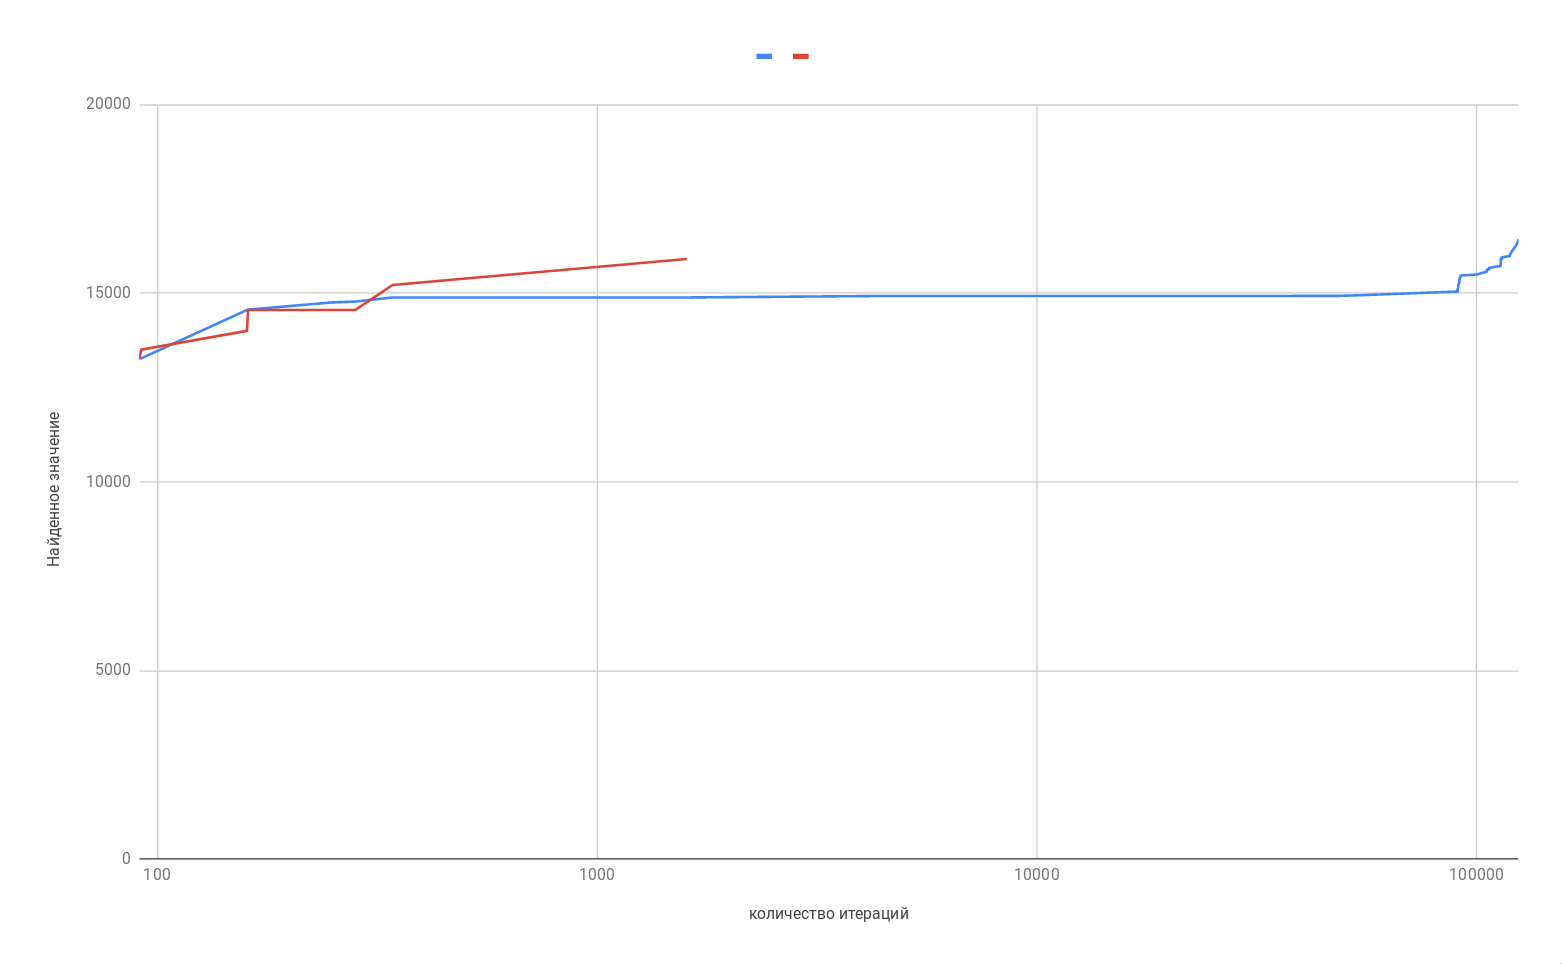
\includegraphics[width=\textwidth]{graph.png}
    Найденные значение: с 5\% погрешности: 15902, без:  16418
\end{frame}

\begin{frame}
\frametitle{Визуализация}
    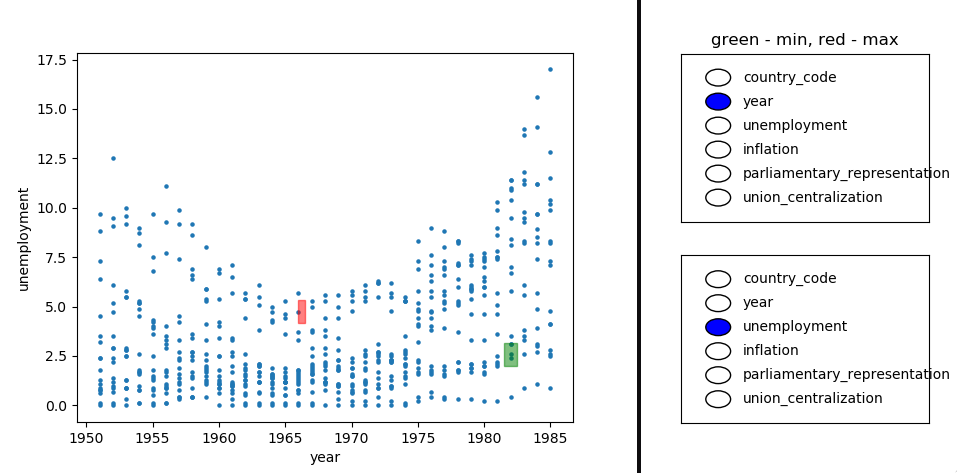
\includegraphics[width=\textwidth]{visual.png}
\end{frame}

\end{document}
